%!TEX root = ../thesis.tex

\chapter*{About the author}
\addcontentsline{toc}{chapter}{About the author}
\markboth{\MakeUppercase About the author}{\MakeUppercase About the author}

\begin{wrapfigure}{r}{0.5\textwidth}
	\vspace{-20pt}
	\centering
	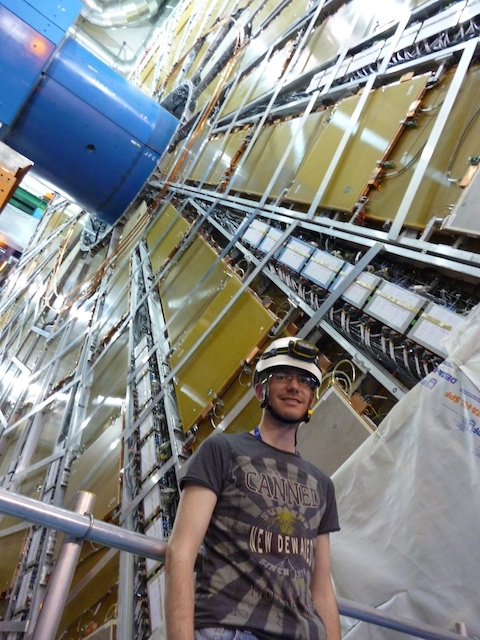
\includegraphics[width=0.48\textwidth]{tex/david_photo}
	\vspace{-20pt}
\end{wrapfigure}

David Hall obtained a first class MPhys degree at the University of Warwick in 2010. For his 
masters research, he developed a prototype for a novel intensity modulated radiotherapy 
treatment modality at the University Hospital in Coventry, under the supervision of Prof.\ 
Adrian Wilson.

David received his DPhil degree in 2014 at the University of Oxford whilst working on the 
ATLAS experiment at CERN. This involved measuring the \WW cross section and searching for 
evidence of the Higgs boson, under the supervision of Dr Chris Hays. He then worked as the 
ATLAS Monte Carlo software coordinator in the preparation for Run-II of the LHC.

In January 2015, David moved into proton therapy research in order to combine his previous 
research experiences, and spent a short time at the Particle Therapy Cancer Research 
Institute, University of Oxford. He is now a postdoctoral research fellow at Massachusetts 
General Hospital and Harvard Medical School. He develops Monte Carlo simulation programs and 
treatment planning systems for proton therapy, in Prof.\ Harald Paganetti's group.

\nocite{HWW-RunI-submit,ATLAS:combination:2013,YR3,ATLAS-discovery2,ATLAS-discovery,WW-7TeV,WW-1ifb,VersatileLinkConnectors,VersatileLinkFibres,VersatileLink}

\let\oldbibname\bibname
\renewcommand{\bibname}{Selected publications}
\bibliographystyle{thesis}
\bibliography{theory,pheno,mc,experiment}
\let\bibname\oldbibname
